\graphicspath{{../../../PhD/paper_factory/thesis_louis/Chapter2/Figs/}{./figs/}}
\subsection{Background}

\begin{frame}[t]
\frametitle{Historical Background of Floating-Point Arithmetic}

% Timeline start and end years

\newcommand{\startyear}{1840}
\newcommand{\endyear}{2025}
\newcommand{\timelineLength}{185}

\tiny
\begin{tikzpicture}[xscale=12 / \timelineLength] % Adjust scale to fit 200 years on the slide
\draw[line width=1mm,-latex,red!20] (-0.2,0) -- (\timelineLength + 0.2,0); % Extended timeline
\foreach \X [count=\Z] in {1840, 1914, 1938, 1954, 1980, 1981, 1985, 2008, 2012, 2015, 2017, 2019, 2022}
{
  % Calculate position based on year
  \pgfmathsetmacro{\YearPos}{(\X-\startyear) / \timelineLength * \timelineLength}
  \ifodd \Z
    \filldraw[highlight on=<\Z>] (\YearPos, 0.05) -- (\YearPos + 0.8, 0.4) -- (\YearPos - 0.8, 0.4) -- cycle; % Triangle pointing up
    \pgfmathsetmacro{\AdjustedXPos}{\YearPos + 2}
    \node[anchor=south, rotate=45, inner sep=2pt] at (\AdjustedXPos, 0.55) {\X}; % Date above triangle
  \else
    \filldraw[highlight on=<\Z>] (\YearPos, -0.05) -- (\YearPos + 0.8, -0.4) -- (\YearPos - 0.8, -0.4) -- cycle; % Triangle pointing down
    \pgfmathsetmacro{\AdjustedXPos}{\YearPos - 2.7}
    \node[anchor=north, rotate=45, inner sep=2pt] at (\AdjustedXPos, -0.55) {\X}; % Date below triangle
  \fi
}
\end{tikzpicture}
\scriptsize
\vspace{-6mm}
\begin{myitemize}
\item<1> 1840: Babbage and Lovelace conceptualize the first floating-point.
\item<2> 1914: Leonardo T. Quevedo builds an electromechanical calculator with floating-point.
\item<3> 1938: Konrad Zuse \textbf{Z1}, the first programmable mechanical computer with floating-point arithmetic.
\item<4> 1954: IBM 704, the first mass-produced computer with floating-point hardware.
\item<5> 1980: Intel introduces the 8087 co-processor.
\item<6-> 1981: \textbf{Kulisch}: "Computer Arithmetic in Theory and Practice"
\item<7> 1985: \textbf{IEEE754}-85 standard.
\item<8> 2008: IEEE754-08 introduces half-precision and FMA
\item<9> 2012: AlexNet sparks the AI revolution with its CNN structure.
\item<10> 2015: Introduction of bfloat16, optimizing neural network computations.
\item<11-> 2017: Introduction of the \textbf{Posit} format, a new take on floating-point representation.
\item<12> 2019: IEEE754 standard evolves to fix errors
\item<13-> 2022: \textbf{LLM revolution}, chatgpt, MX format (e2m2, e4m3, e5m2), tensor cores
\end{myitemize}

	\only<14>{}

\normalsize
\end{frame}


\begin{frame}[t]
\frametitle{Timeline Zoom: "LLM Revolution"}

% Define start and end years
\newcommand{\startyear}{2018}
\newcommand{\endyear}{2025}
\newcommand{\timelineLength}{7} % Total length of the timeline in years

\only<1-8>{
\vspace{-3mm}
\tiny
\begin{tikzpicture}[xscale=1.5] % Adjust scale for better visualization
% Draw the main timeline with extended arrows
\draw[line width=1mm, -latex, red!20] (-0.0, 0) -- (\timelineLength + 0.4, 0);

% Draw year markers and divide each year into 12 segments (months)
\foreach \year in {0,...,\timelineLength} {
    \pgfmathsetmacro{\yearValue}{int(\startyear + \year)} % Calculate year value
    \draw[thin] (\year, -0.1) -- (\year, 0.1); % Draw year ticks
    \node[anchor=north] at (\year, -0.2) {\yearValue}; % Label the year

    % Draw month markers between each year except the last year
    \ifnum\year<\timelineLength
        \foreach \month in {1,...,11} {
            \pgfmathsetmacro{\monthPos}{\year + \month / 12}
            \draw[thin, gray] (\monthPos, -0.05) -- (\monthPos, 0.05); % Draw month ticks
        }
    \fi
}

% Position events based on the exact month and year, and move the red triangle
\foreach \date/\label [count=\Z] in {
    2018.50/Jun 2018,%: Posit draft evolves,
    2020.92/Dec 2020,%: MSFP,
    2021.67/Sep 2021,%: Unum-IV,
    2021.83/Oct 2021,%: Tesla Cfloat8/16,
    2022.25/Mar 2022,%: Posit becomes standard,
    2023.50/Jun 2023,%: Bfloat16 subnormals,
    %2023.50/Jun 2023,%: MXFP formats,
    %2023.50/Jun 2023,%: OCP 8-bit FP,
    2023.75/Sep 2023,%: OCP announcement,
    %2023.75/Sep 2023,%: IEEE P3109,
    2024.42/May 2024%: PT-Float,
    %2024.42/May 2024,%: IEEE P3109 new formats
} {
    % Draw a moving red triangle based on list item highlighting
    \filldraw[red, highlight on=<\Z>] (\date - \startyear, 0.06) -- ++(0.1, 0.4) -- ++(-0.2, 0) -- cycle;
    % Only show minimal month/year labels on the timeline
    \node[anchor=south, rotate=45, inner sep=2pt] at (\date - \startyear+0.22, 0.76) {\label};
}

\end{tikzpicture}
	%\vspace{10pt}

\scriptsize
\vspace{-2mm}
\begin{myenumerate}
    %\item<1-> June 2018: Posit draft evolves.
    %\item<2-> December 2020: Microsoft Floating-Point (MSFP) presented at NeurIPS~\cite{rouhani_pushing_2020}.
    %\item<3-> September 2021: Proposal for Unum-IV~\cite{serodio2021unum}.
    %\item<4-> October 2021: Tesla Dojo Cfloat8 and Cfloat16~\cite{talpes_dojo_2022}.
    %\item<5-> March 2022: Posit draft becomes a standard.
    %\item<6-> June 2023: Some Bfloat16 include subnormals.
    %\item<6-> June 2023: MXFP formats (MXFP8: E5M2, E4M3; MXFP6: E3M2, E2M3; MXFP4: E2M1) and MXINT8 introduced as "block formats" at ISCA~\cite{darvish_rouhani_shared_2023}.
    %\item<6-> June 2023: OCP 8-bit Floating-Point Specification.
    %\item<7-> September 2023: OCP announcement~\cite{rouhani_microscaling_2023}
    %\item<7-> September 2023: IEEE Working Group P3109 introduces report on 8-bit FP formats.
    %\item<8-> May 2024: Introduction of PT-Float at ARITH 2024~\cite{sousa2024ptfloat}.
    %\item<8-> May 2024: IEEE Working Group P3109 mentions 28 new formats.
    \item<1-> Jun 2018: Posit draft evolves.
    \item<2-> Dec 2020: MSFP at NeurIPS~\cite{rouhani_pushing_2020}.
    \item<3-> Sep 2021: Unum-IV~\cite{serodio2021unum}.
    \item<4-> Oct 2021: Tesla Cfloat8/Cfloat16~\cite{talpes_dojo_2022}.
    \item<5-> Mar 2022: Posit draft becomes a standard.
    \item<6-> Jun 2023: Bfloat16 with subnormals.
    \item<6-> Jun 2023: MXFP formats & MXINT8~\cite{darvish_rouhani_shared_2023}.
    \item<6-> Jun 2023: OCP 8-bit FP spec.
    \item<7-> Sep 2023: OCP announcement~\cite{rouhani_microscaling_2023}.
    \item<7-> Sep 2023: IEEE P3109 report on 8-bit FP.
    \item<8-> May 2024: PT-Float at ARITH 2024~\cite{sousa2024ptfloat}.
    \item<8-> May 2024: IEEE P3109: 28 new formats.

\end{myenumerate}

\normalsize
\only<1>{Approximate number of new float formats: \fbox{ 5}}
\only<2>{Approximate number of new float formats: \fbox{11}}
\only<3>{Approximate number of new float formats: \fbox{12}}
\only<4>{Approximate number of new float formats: \fbox{14}}
\only<5>{Approximate number of new float formats: \fbox{19}}
\only<6>{Approximate number of new float formats: \fbox{32}}
\only<7>{Approximate number of new float formats: \fbox{32}}
\only<8>{Approximate number of new float formats: \textbf{\fbox{53}}}

}
%\begin{frame}
%\frametitle{Another concern addressed by this thesis}
\only<9->{
\begin{alertblock}<9->{Modern history emphasizes "Arithmetic wall"}
    %\vspace{-6mm}
	The "LLM revolution" introduces dozens of formats. SOTA constantly evolves and standards now specify \textbf{meta-formats}.
\end{alertblock}
\begin{block}<10->{Another concern addressed by this thesis}
	This thesis tackles this issue through \textbf{format-agnosticism}. Contributions are \textbf{succesfully re-evaluated} using recent SOTA.
    %\vspace{-6mm}
\end{block}
	}

\end{frame}

\begin{frame}
    \frametitle{Background: Kulisch Accumulation}

        \begin{itemize}
	   \item<1-> \textbf{Exact accumulator}.
	   \item<1-> Fixed-point circuitry $\Rightarrow$ \textbf{One bit per binade}.
	   \item<1-> \textbf{Easy pipelining:} One branch accumulation.
           \item<1-> Shift in place the addend.
           \item<1-> Postpones rounding.
	   \item<1-> \textbf{Fused} summation and dot product.
        \end{itemize}
	\begin{block}<2->{Cost consideration}
		IEEE754-64 \textbf{exact} accumulation of product requires over \textbf{4000 bits}.
		\textbf{Never adopted by the standard}.
	\end{block}

\end{frame}

\begin{frame}
    \frametitle{Comparison of Accumulation Methods}

    % Show first image on the first slide
    \only<1>{
        \begin{figure}[H]
            \centering
            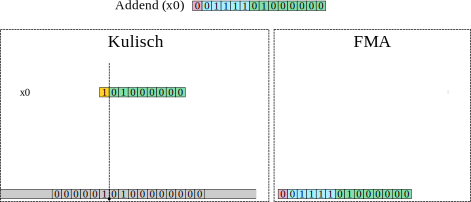
\includegraphics[width=0.8\textwidth]{kulisch1.pdf}
            %\caption{Description for Image 1}
        \end{figure}
    }

    % Show second image on the second slide
    \only<2>{
        \begin{figure}[H]
            \centering
            \includegraphics[width=0.8\textwidth]{kulisch2.pdf}
            %\caption{Description for Image 2}
        \end{figure}
    }

    % Show third image on the third slide
    \only<3>{
        \begin{figure}[H]
            \centering
            \includegraphics[width=0.8\textwidth]{kulisch3.pdf}
            %\caption{Description for Image 3}
        \end{figure}
    }

    % Show fourth image on the fourth slide
    \only<4>{
        \begin{figure}[H]
            \centering
            \includegraphics[width=0.8\textwidth]{kulisch4.pdf}
            %\caption{Description for Image 4}
        \end{figure}
    }
    \only<5->{
        \small
         \begin{exampleblock}<5->{Results}
            \vspace{-6mm}
            \begin{align*}
                R_\text{exact} &= 46.89794921875 \\
                R_\text{FMA} &= 4\color{red}{5.4375} \\
                R_\text{Kulisch} &= 46.89794921875
            \end{align*}
            %\vspace{-12mm}
        \end{exampleblock}

    %    \begin{alertblock}<6->{Error Analysis and Formulas}
    %        \vspace{-6mm}
    %        \begin{align*}
    %            \text{Absolute Error} &= |R_\text{exact} - R| \\
    %            \text{Relative Error} &= \frac{|R_\text{exact} - R|}{|R_\text{exact}|}
    %        \end{align*}

    %        %\vspace{-4mm}
    %        \begin{table}[H]
    %            \centering
    %            \begin{tabular}{|c|c|c|}
    %                \hline
    %                & \textbf{Absolute Error} & \textbf{Relative Error} \\ \hline
    %                \textbf{FMA} & 1.46044921875 & 0.0311 (3.11\%) \\ \hline
    %                \textbf{Kulisch} & 0 & 0 \\ \hline
    %            \end{tabular}
    %        \end{table}
    %    \end{alertblock}
    }
    %\normalsize
\end{frame}



%\begin{frame}
%    \frametitle{Background: Posit format}
%	\begin{columns}
%	\begin{column}{0.5\textwidth}
%		\begin{itemize}
%			\item TEMP
%		\end{itemize}
%	\end{column}
%	\begin{column}{0.5\textwidth}
%    \begin{figure}[H]
%    \centering
%    \begin{figure}{0.65\textwidth}
%        \centering
%        \includegraphics[width=\linewidth]{Chapter2/Figs/posit_16_4_bit_pattern.pdf}
%        \caption{Bit pattern with all components}
%    \end{figure}
%    \\
%    %\hfill
%    \begin{figure}{0.65\textwidth}
%        \centering
%        \includegraphics[width=\linewidth]{Chapter2/Figs/posit_16_4_bit_pattern_no_frac.pdf}
%        \caption{Without fraction}
%    \end{figure}
%    \\
%    \begin{figure}{0.65\textwidth}
%        \centering
%        \includegraphics[width=\linewidth]{Chapter2/Figs/posit_16_4_bit_pattern_no_frac_no_scale.pdf}
%        \caption{Without fraction and scale}
%    \end{figure}
%    \\
%    %\hfill
%    \begin{figure}{0.65\textwidth}
%        \centering
%        \includegraphics[width=\linewidth]{Chapter2/Figs/posit_16_4_bit_pattern_no_frac_no_scale_no_terminating.pdf}
%        \caption{Without fraction, scale, terminating bit}
%    \end{figure}
%	\end{column}
%\end{figure}
%
%\end{frame}

\begin{frame}
    \frametitle{Background: Posit format}
    \begin{columns}
        \begin{column}{0.45\textwidth}
            \begin{itemize}
		\item<1-> \textbf{``Tapered-Precision''} Posit$\left \langle N,es \right \rangle$.
		\item<1-> N the bitwidth, es exponent size.
		\item<2-> \textbf{Variable-Lenght} fields.
		\item<2-> \textbf{Golomb Rice} regime (r).
		\item<2-> \textbf{Regime} is super-exponent
		\item<3-> \textbf{Quire:} Kulisch in standard.
		\item<3-> \textbf{Claim} to replace \textit{IEEE754}
		\item<3-> \textbf{1} NaN
		\item<3-> \textbf{Dynamic Range} enhanced
		\item<3-> \textbf{Precision around one} enhanced
            \end{itemize}
        \end{column}
        \begin{column}{0.55\textwidth}
		\begin{figure}[H]
            \centering
			\vspace{5pt}
            \includegraphics[width=0.9\textwidth]{posit_16_4_bit_pattern.pdf}
			\vspace{-10pt}
            \caption{All components}

            \includegraphics[width=0.9\textwidth]{posit_16_4_bit_pattern_no_frac.pdf}
			\vspace{-10pt}
            \caption{Without fraction}

            \includegraphics[width=0.9\textwidth]{posit_16_4_bit_pattern_no_frac_no_scale.pdf}
			\vspace{-10pt}
            \caption{Without fraction and scale}

            \includegraphics[width=0.9\textwidth]{posit_16_4_bit_pattern_no_frac_no_scale_no_terminating.pdf}
			\vspace{-10pt}
            \caption{Only regime}
	\end{figure}
        \end{column}
    \end{columns}
\end{frame}


